\let\negmedspace\undefined
\let\negthickspace\undefined
\documentclass[journal,12pt,onecolumn]{IEEEtran}
\usepackage{cite}
\usepackage{amsmath,amssymb,amsfonts,amsthm}
\usepackage{algorithmic}
\usepackage{graphicx}
\graphicspath{{./figs/}}
\usepackage{textcomp}
\usepackage{xcolor}
\usepackage{txfonts}
\usepackage{listings}
\usepackage{enumitem}
\usepackage{mathtools}
\usepackage{gensymb}
\usepackage{comment}
\usepackage{caption}
\usepackage[breaklinks=true]{hyperref}
\usepackage{tkz-euclide} 
\usepackage{listings}
\usepackage{gvv}                                        
%\def\inputGnumericTable{}                                 
\usepackage[latin1]{inputenc}     
\usepackage{xparse}
\usepackage{color}                                            
\usepackage{array}
\usepackage{longtable}                                       
\usepackage{calc}                                             
\usepackage{multirow}
\usepackage{multicol}
\usepackage{hhline}                                           
\usepackage{ifthen}                                           
\usepackage{lscape}
\usepackage{tabularx}
\usepackage{array}
\usepackage{float}
\newtheorem{theorem}{Theorem}[section]
\newtheorem{problem}{Problem}
\newtheorem{proposition}{Proposition}[section]
\newtheorem{lemma}{Lemma}[section]
\newtheorem{corollary}[theorem]{Corollary}
\newtheorem{example}{Example}[section]
\newtheorem{definition}[problem]{Definition}
\newcommand{\BEQA}{\begin{eqnarray}}
\newcommand{\EEQA}{\end{eqnarray}}
\newcommand{\define}{\stackrel{\triangle}{=}}
\theoremstyle{remark}
\newtheorem{rem}{Remark}

\begin{document}

\title{10.7.104}
\author{ee25btech11056 - Suraj.N}
\maketitle
\renewcommand{\thefigure}{\theenumi}
\renewcommand{\thetable}{\theenumi}

\begin{document}

\textbf{Question :} Let \(a,b\) and \(\lambda\) be positive real numbers. Suppose \(P\) is an end point of the latus rectum of the parabola \(y^2=4\lambda x\), and suppose the ellipse \(\dfrac{x^2}{a^2}+\dfrac{y^2}{b^2}=1\) passes through the point \(P\). If the tangents to the parabola and the ellipse at the point \(P\) are perpendicular to each other, then the eccentricity of ellipse is 

\textbf{Solution :}

\begin{table}[h!]
  \centering
  \begin{tabular}{|c|c|}
\hline
\textbf{Name} & \textbf{Value} \\
\hline
Circle & $\vec{x}^\top\vec{x} - a^2 = 0$ \\
\hline
Line & $\vec{x} = \myvec{\tfrac{a}{\sqrt{2}} \\ 0} + \kappa\myvec{0 \\ 1}$ \\
\hline
\end{tabular}

  \caption*{Table : Parabola and Ellipse}
  \label{10.7.104}
\end{table}

The parameters of the parabola are :

\begin{align}
  \vec{V_1} &= \myvec{0 & 0\\0 & 1} & \vec{u_1} &= \myvec{-2\lambda\\0} & f_1 &= 0
\end{align}

The parameters of the ellipse are :

\begin{align}
  \vec{V_2} &= \myvec{\tfrac{1}{a^2} & 0\\0 & \tfrac{1}{b^2}} & \vec{u_2} &= \vec{0} & f_2 &= -1 \label{eq:ellipse} 
\end{align}

The end point of the latus rectum of parabola is 

\begin{align}
  \vec{P} &= \myvec{\lambda\\2\lambda}
\end{align}

The equation of tangent to the parabola at $\vec{P}$ is given as :

\begin{align}
  (\vec{V_1}\vec{P}+\vec{u_1})^\top\vec{x} + \vec{u_1}^\top\vec{P} + f_1 &= 0 & \vec{n_1} &= \vec{V_1}\vec{P}+\vec{u_1} 
\end{align}

The equation of tangent to the ellipse at $\vec{P}$ is given as :

\begin{align}
  (\vec{V_2}\vec{P}+\vec{u_2})^\top\vec{x} + \vec{u_2}^\top\vec{P} + f_2 &= 0 & \vec{n_2} &= \vec{V_2}\vec{P}+\vec{u_2} 
\end{align}

\pagebreak

As the tangents at $\vec{P}$ are perpendicular , the normal vectors of the tangents are also perpendicular 

\begin{align}
  \vec{n_1}^\top\vec{n_2} = 0\\
  (\vec{V_1}\vec{P}+\vec{u_1})^\top\vec{V_2}\vec{P} = 0\\
  (\vec{P}^\top\vec{V_1}^\top+\vec{u_1}^\top)\vec{V_2}\vec{P} = 0\\
  \myvec{-1 & 1}\myvec{\tfrac{1}{a^2} & 0\\0 & \tfrac{1}{b^2}}\myvec{1\\2} = 0\\
  \frac{a^2}{b^2} = \frac{1}{2} \label{eq:ab} 
\end{align}

From \eqref{eq:ellipse} , the eigen values of $\vec{V_2}$ are the diagonal entries as it is an upper triangular matrix and also $a<b$

\begin{align}
  \lambda_1 &= \frac{1}{b^2} & \lambda_2 &= \frac{1}{a^2}
\end{align}

The eccentricity e of ellipse is given as 

\begin{align}
  e = \sqrt{1 - \frac{\lambda_1}{\lambda_2}}\\
  e = \sqrt{1 - \frac{a^2}{b^2}}
\end{align}

From \eqref{eq:ab} , we get 

\begin{align}
  e = \frac{1}{\sqrt{2}}
\end{align}

\pagebreak

\begin{figure}[h!]
  \centering
  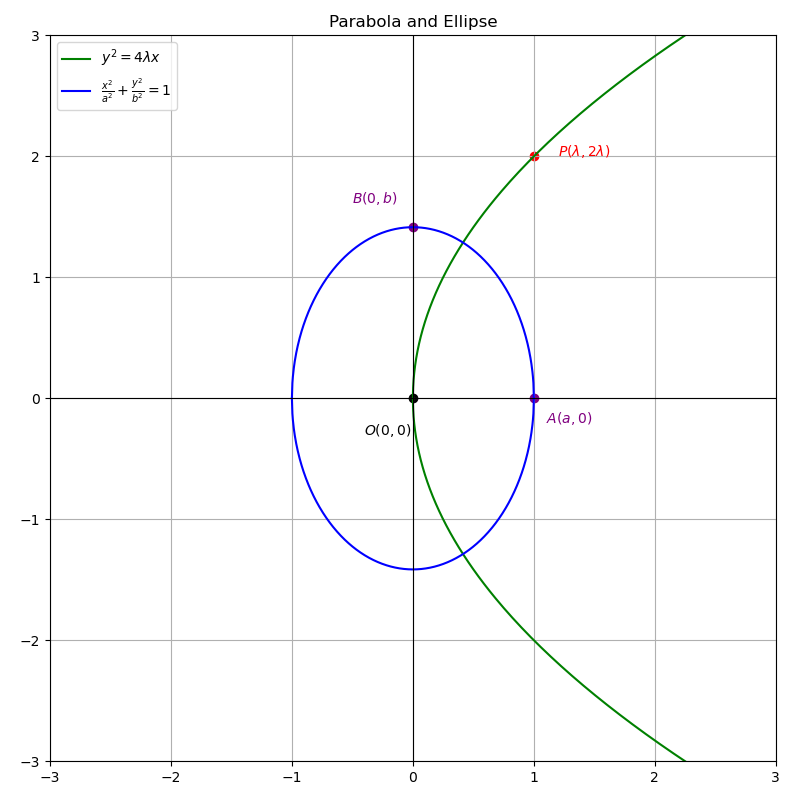
\includegraphics[width=0.7\columnwidth]{figs/parabola_ellipse.png} 
   \caption*{Fig : Parabola and Ellipse}
  \label{Fig1}
\end{figure}

\end{document}

